\documentclass{article}
\usepackage[utf8]{inputenc}

\title{Tsai Thesis Notes}
\author{Robert Twyman}
\date{October 2018}

\usepackage{natbib}
\usepackage{graphicx}
\usepackage{xcolor}

\begin{document}

\maketitle

This document will be my notes of Tsai's Thesis \cite{Tsai2018TsaiEfc.pdf}

\section{Abstract - Page 3}
\subsection{Aims of the thesis}
\begin{itemize}
\item General aim of PET research is to improve the quantitative consistency in reconstruction of PET images without compromising the patient through practice.
\item To improve the quantitative consistency in reconstruction of PET images.
\item L-BFGS-B-PC performance in simulation and three patient datasets allows for several times faster convergence than SPS
\item L-BFGS-B-PC - less sensitive to penalty type, penalty strength, noise level, and background level compared to L-BFGS-B
\item \textbf{Anatomical penalty function is considered with a spatially-variant penalty strength}
\begin{itemize}
\item \color{red}{a function which varies over space (based on CT?)}
\item \textbf{reduces the quantitative dependence on surrounding activity and location}
\item In addition to algorithm convergence rate and consistency improvements.
\end{itemize}
\item Misalignment considered between function and anatomical images.
\end{itemize}
\section{Introduction - Page 25}
\begin{itemize}
\item Reconstructed images expected to accurately represent tracer concentration.
\item General aim, make "good" images from PET data for clinical reconstruction timescales when auxiliary information (CT data) is available.
\end{itemize}

\section{Background}
\subsection{Emission Tomography  - Page 27}
\begin{itemize}
\item Non-invasive observations of metabolic processes in vivo
\begin{itemize}
\item allows for valuable diagnosis of many diseases.
\end{itemize}

\item \textbf{Radioactive tracers} 
\begin{itemize}
\item one atom in the molecule injected is a radioactive isotope
\item The tracers are designed to be used in physiological processes

\item Dependant on the isotope and decay, photons or positions (beta +) are emitted during the decay process. 
\item A scanner/ detector is used for specific types of emission
\item SPECT - Single Photon Emission Computer Tomography - uses a decay process which involves a single photon emission.
\item PET - Position Emission Tomography - uses a beta plus decay which leads to position-electron annihilation.
\end{itemize}
\end{itemize}

\subsubsection{Current/ potential clinical applications  - Page 28}
\begin{itemize}
\item Oncology - $^{18}$F-FDG (fluorodeoxy-glucose) - a common tracer used in PET. It reflects the high metabolism rate of glucose in malignant cells.
\item Cardiology - $^{201}$Tl in SPECT and $^{13}$N-ammonia in PET are tracers that can be used in myocardial perfusion studies help to diagnose coronary artery disease and heart muscle damage. Cells with low/no uptake of tracer uptake and therefore analysis of SPECT/PET images can lead to diagnosis.
\item Neurology - $^{99m}$Tc-HMPAO (hexamethylpropyleneamineoxime) (SPECT) and $^{11}$C-PiB (Pittsburgh Compound-B) or related $^{18}$F tracers (PET) - can be used in the examination of Alzheimer's and Parkinson's disease. These tracers can transverse the blood brain barrier.
\end{itemize}

\subsubsection{Scanners and principles - Page 29}
\begin{itemize}
\item \textbf{SPECT}  
\begin{itemize}
\item radioisotope decays into a $\gamma$-ray. The SPECT imaging system usually consist of multiple detector heads rotated round a patient to obtain projections from angles around the target. $\gamma$-rays are emitted with no preference in direction so physical collimators are required to limit the incidence angle of rays. 
\item While this improves spatial resolution of each projection angle, {\color{red}it does lower sensitivity?} 
\end{itemize}

\item \textbf{PET} 
\begin{itemize}
\item (radioisotopes) undergo beta plus $\beta ^+$decay into a position. 
\item The position proceeds to lose its kinetic/thermal energy via coulomb scatter until it annihilates with an election. 
\item This annihilation process creates two photons, emitted back to back in the center of mass frame. Since the electron/position pair may not be at rest at time of annihilation, some kinetic energy may reside leading to non-back-to-back scatter. 
\end{itemize}The position proceeds tPhotons are detected and are recorded as an event by a detector. 
\item A line of response (\textbf{LOR}) can be traced as a straight line between two detectors if two events are deemed a coincidence.
\item In PET, detectors are stationary in a ring shape achieving multiple angle acquisition.
\item A pair of parallel detector ring along the transaxial direction and sometimes a thin septa of lead/tungsten to block coincidences lying in different detector rings. outside the predefined ring difference.o lose its kinetic/th

\item \textbf{DETECTORS}
\begin{itemize}
\item $\gamma$-rays/ annihilation photons in (both systems) use scintillation crystals (scintillator). These absorb high energy photons and readmit lower energy (optical) photons.
\item Scintillators are coupled with a detector for optical photons (such as photo-multiplier tubes (PMT) and silicon photo-multiplier tubes (SiPMs)
\item The optical photons are then converted to electrical signals which leads to Data acquisition.
\end{itemize}
\end{itemize}

\subsubsection{Data acquisition - Page 30}
\begin{itemize}
\item The ring shaped arrangement of a PET scanner allows for simultaneous acquisition of events at various angles.
\item PET data acquisition can be done in 2D or 3D
\item annihilation photons detected by different rings are blocked by a high-Z element septa
\item \textbf{3D} - the septa is removed to improve detection sensitivity and so LORs across different rings are acceptable for for simultaneous acquisition of events at various angles.
\item \textbf{Types of Event}
\begin{itemize}
\item Valid event - 2 photons genertated from the same annihilation event are detected in a pair of detectors within a specified timing window and DO NOT have any other interations.
\item Scattered event - one or both photons from an annihilation event are scattered (have their direction changed) via Compton scattering processes with any object along their path. These are rejected with the aid of an energy discriminator (i.e. if the energy low is greater than a threshold/acceptable amount). If the energy is bellow threshold but is scattered, this can lead to mispossitioning of the event.
\item Random event - caused by two accidental photons from unrelated annihilation events in a pair of detectors within the coincidence timing window. This can lead to mispositioning as the apparent LORs are far from the true locations.
\item $\textbf{g} = \textbf{g}^{valid} + \textbf{g}^{scattered} + \textbf{g}^{randoms}$
\end{itemize}
\end{itemize}

\subsubsection{Data Organization}
2D data
\begin{itemize}
\item coordiante system w.r.t the detector is introduced
\item $(r,s)$
\item Given the data collection angle $\phi$, we can determine the transform from an $(x,y)$ system with $ r = x cos(\phi) + y sin(\phi) $ and $ s = x cos(\phi) - y sin(\phi) $
\item  \textbf{FOR SPECT} - Data is recorded in the form of a \textit{sinogram} matrix
\begin{itemize}
\item (as a sinusoidal path is observed down the matrix) 
\item a 2-D matrix $\textbf{p}(r,\phi)$   
\item the relationship between the matrix element 
$p(r,\phi)$
and the tracers distribution on the 
$\textit{(x,y)}$
coordinate system is given by:
\end{itemize}
\end{itemize}
\[  
\textbf{p}(r,\phi) = 
\int _{-\infty}^{\infty} 
    f(
        r\cos\phi - s\sin\phi, 
        r\sin\phi + s\cos\phi)
    )ds
\]
\begin{itemize}
\item 
\begin{itemize}
\item for 3D volumes, the data organization is a stack of sinograms that record projections for each slice in \textit{z} in the FOV
\end{itemize}
\item \textbf{FOR PET} (\textit{Similar to SPECT but with an extra step}
\begin{itemize}
\item As PET scanners recorded every event instead of projections from different angles an extra step is required.
\item Specific time frames, events are accumulated and combined with adjacent parallel LORs to represent projection data from a particular angle.
\item In 2D, the following steps are identical to the SPECT steps (when physical steps are not involved)
\item 3D data is collected as a stack of sinograms with additional sinograms representing projections at different polar angle $\theta$  Figure.\ref{3D Coordinate system PET}
\end{itemize}
\end{itemize}
\begin{figure}{\linewidth}
	\centering
	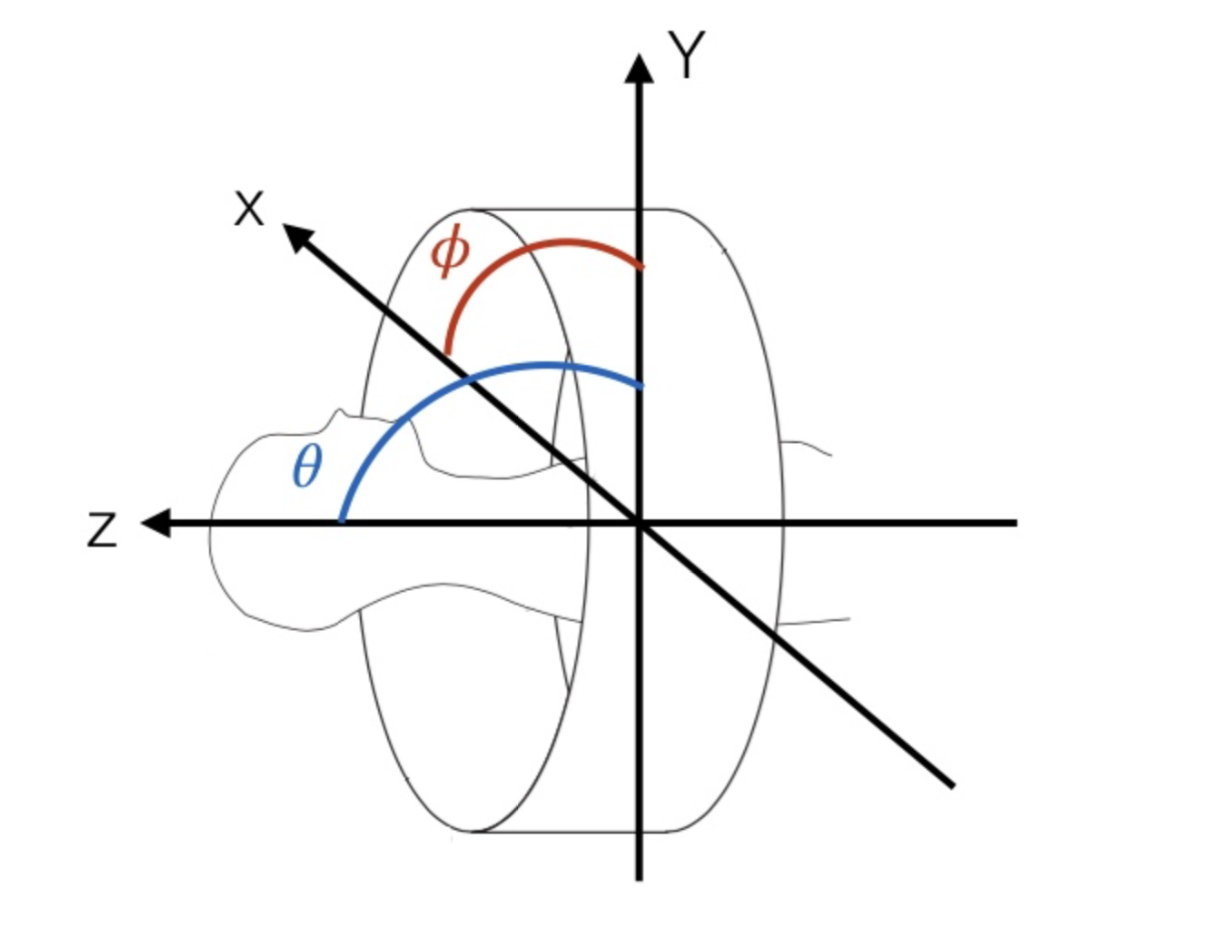
\includegraphics[width = \linewidth]{Tsai's Thesis Analysis/3D Coordinate system for PET.png}
    \caption{\label{3D Coordinate system PET}}
\end{figure}
\subsubsection{Attenuation effect and correction}
\begin{itemize}
\item The scattered/attenuated data will not reflect true tracer activity
\item The probability of detection depends on path and materials that the $\gamma$-ray photons take. 
\item The measured PET data for a single slice, considering the attenuation effects, is:
\end{itemize}
\[ 
p(r,\phi) = 
\int_{-\infty} ^{\infty} 
    f(r\cos\phi - s\sin\phi, r\sin\phi + s\cos\phi) 
e^{
    f(r\cos\phi - s'\sin\phi, r\sin\phi + s'\cos\phi)ds'
}ds
\]
\begin{itemize}
\begin{itemize}
\item If there is no correction for attenuation then the images reconstructed from the data cannot represent true activity.
\item High density tissues (ie bone) lead to high attenuation and so artifacts in images
\item Information from CT/MR scans can help with anatomical information
\end{itemize}
\end{itemize}

\subsection{CT  - Page 36}
\begin{itemize}
\item CT, provide insight into structural detail regarding tissue size, location and morphological change. Moreover, anatomical information can be used for performing attenuation correction in PET.
\item Typical CT x-ray tubes can produce photons with energies 20-150 keV
\item \textbf{CT image generation}
\begin{itemize}
\item x-ray absorption measured in Hounsfield Units (HU) and is based upon a scaled attenuation correction
\item  $ HU = 1000 \times \frac{\mu - \mu_{water}}{mu_{water} - \mu_{air}}$
\end{itemize}
\end{itemize}
\section{PET Image Reconstruction  - Page 38}
\subsection{Back projection (BP) and Filtered Back Projection (FBP)}
\begin{itemize}
\item \textbf{Basic Back Projection - BP}
\item events stored in each sinogram are back projected along the path they are collected from (in the discrete image plane).
\item However this leads to every pixel sharing the total accumulated events (ie outside the body has events projected)
\item The projections at different angles are combine to form a tracer distribution $f(x,y)$ (ie a pet image)
\item These image are blurred.
\item \textbf{Filtered Back Projection - FBP}
\item A ramp filter is applied to the back projection to compensate for blurring effects due to the back projection
\item FBP has limitations such as 
\begin{itemize}
\item artifacts if acquisition is incomplete
\item Streaks artifact can be observed for few event data sets.
\item FBP algorithms cannot be modified to account for physical effects of the imaging system
\end{itemize}
\end{itemize}
\subsection{Iterative algorithms - Page 39}
Iterative reconstruction algorithms are the method of choice in ET. These methods allow for more reliable quantification based on the resulting image by adopting successive estimates towards a solution based upon the objective function
\subsubsection{Model}
\[\vec{\textbf{g}} = \textbf{A}\textbf{f} + \textbf{n}\]
$\textbf{f} = [f_1, ... , f_J]^T $ - the discrete tracer distribution 
$\textbf{n} = [n_1, ... , n_I]^T $ - the expected \textbf{invalid} events
$\vec{\textbf{g}} = [g_1, ... , g_I]^T $  - the statistical mean of the observed data
$\textbf{A}$ is a $I \times J$ transition (or system) matrix, each element $A_{ij}$ indicates the probability of an emission from the voxel j is detected by detector bin $i$ without scatter. bin \textit{i} referrers to the $i^{th}$ element of the sinogram. This matrix characterises the physical system properties, such as resolution and detector sensitivity, in terms of detection probability.

\subsubsection{Objective function  - Page 39}
\textit{The function you wish to maximise or minimise and in image reconstruction, the difference between the measured and estimated data}

For ET,  the prob of collecting data $\textbf{g}$ given a tracer distribution $\textbf{f}$ is given by a Poisson model.

The typical Poisson model gives the probability of $k$ based upon $\lambda$
\[
P(\lambda,k) = 
\frac{e^{-\lambda} \lambda^{-k}}{k!}
\]
$P$ - Probability 
$\lambda$ - mean events per interval
$k$ - probability of an event at particular interval (ie $k = 0,1,2,3,...$)

In PET, we can reorganise this to give us the probability of collecting data
\[
\textbf{P}(\textbf{f},\textbf{g}) = 
\prod_{i=1}^{N}
\frac{e^{-\vec{g}_i} g_i^{-g_i}}{k!}
\]
$\vec{g}_i$ - the observed mean of the $i^{th}$ bin/detector
$g_i$ - the probability of the event
Note: this version multiplies the probabilities to form a "net" probability and is a vector

The probability function of \textbf{g} can be interpreted as a likelihood function of \textbf{f}. Maximising the probability function (above) is equivalent to finding an estimate of the distribution $\hat{\textbf{f}}$ that give the maximum likely-hood. This process is called \textbf{Maximum-Likelihood (ML)}.

Take the log of this (omit terms independent of \textbf{f}) to get \textbf{log-likelihood} estimation function

\[
L(\textbf{f},\textbf{g}) = 
\sum_i g_i \log \vec{g}_i (\textbf{f}) - \vec{g}_i (\textbf{f})
\]
Maximising $L$ is analogous to minimising $-L$ so it referred to in the thesis as a minimisation problem. 

Image reconstruction using maximum likelihood is an ill-conditioned problem - this means that noise is amplified with iteration. 
Early termination can be used to control the noise at the expense of quantitative accuracy.

Penalty terms can be incorporated also to control noise. Penalised Maximum Likelihood (\textbf{PML}) image reconstruction aims to minimise an objective function $\Phi$ that consists of the negative log-likelihood $-L$ and a \textbf{penalty function} $R$ with a \textbf{strength parameter} $\beta$ in-front.
\[
\Phi(\textbf{f}) = -L(\textbf{f},\textbf{g})  + \beta R(\textbf{f})
\]
The optimisation of this becomes
\[
\hat{\textbf{f}} = 
\arg \min_{\textbf{f}\geq 0} \phi (\textbf{f})  
\]
A positivity constraint is imposed on $\textbf{f}$ as radioactivity density must be greater than or equal to 0. 

\subsection{Penalty functions R}
Penalty term (aka prior?)
Most common is \textbf{Gibbstype} - penalizes the difference between voxels in a given neighbourhood $N$ .
\[
R(\textbf{f}) =
\frac{1}{2} \sum_j \sum_{k\in N_j} \omega_{jk} \phi(f_j - f_k) 
\]
$\omega_{jk}$ - weight between voxel j and its neighbouring voxel k. 
There are two simple potential functions $\phi$:
\begin{itemize}
\item \textbf{Quadratic Penalty - (QP) }- smoothing function which tends to reduce the difference between pixels \textbf{regardless} of the presence of \textbf{true} edges
\[
\phi_{QP}(x) = x^2
\]
\end{itemize}
\begin{itemize}
\item \textbf{Re-scaled log-cosh penalty (LP)} - better at edge preserving than QP
\end{itemize}
\[
\phi_{LP}(x) = 
\frac{1}{\rho^2} \log(\cosh(\rho x)) 
\]
$\rho$ - a scalar controlling the edge preservation of $\phi_{LP}$ 
$\frac{1}{\rho^2}$ - is derived from the \textit{second derivative} of $\phi_{LP}$ and is used for normalisation so both penalties are similar for small values of $|x|$ 

Other regularisation functions include those derived from CT or MR images. These may improve edge delineation of objects in studies. 

\textbf{Joint Total Variation (JTV} - explores edge information based on magnitude of image gradients for both functional ET and anatomical images. The ET implementation incorporates structural details during image reconstruction. This is further improved by consideration of the direction of the gradients.

With the added direction information, the proposed \textbf{Parallel Level Sets (PLS)} shows higher reliability of discovering the structural similarity between these two images.

\textbf{Parallel Level Sets (PLS) is the representative anatomical penalty in this thesis}
\[
\textbf{R}(\textbf{f}|\textbf{z}) = 
\sum_j \sqrt{ \epsilon^2 || [\nabla \textbf{f}]_j ||_2^2 - ([\nabla \textbf{f}]_j \cdot [\xi]_j)^2}
\]
\[
[\xi]_j :=  \frac{[\nabla \textbf{z}]_j}{\sqrt{ ||[\nabla \textbf{z}]_j||_2^2 + \eta^2 }},
\epsilon \text{ and }  \eta >0
\]
$\nabla$ - Gradient operator
$\cdot$ - scalar product
$\textbf{z} = [z_1,...,z_J]^T \in \mathbb{R}$ - is the anatomical image
$||\cdot||_2$ denotes the L2 normalisation 

The edge persevering property of these are preserved by $(\epsilon, \eta)$ 

\subsubsection{MINI-SUMMARY OF OPTIMISATION THUS FAR}
We want to minimise the objective function:
\[\Phi(\textbf{f}) = -L(\textbf{f},\textbf{g})  + \beta \textbf{R}(\textbf{f})\]
where the log-likelihood estimation is given as:
\[ L(\textbf{f},\textbf{g}) = \sum_i g_i \log \vec{g}_i (\textbf{f}) - \vec{g}_i (\textbf{f}) \]
and the PLS (Parallel Level Sets) is given as:
\[
\textbf{R}(\textbf{f}|\textbf{z}) = 
\sum_j \sqrt{ \epsilon^2 || [\nabla \textbf{f}]_j ||_2^2 - ([\nabla \textbf{f}]_j \cdot [\xi]_j)^2}
\]
with the anatomical data $\textbf{z}$ 
\[ [\xi]_j :=  \frac{[\nabla \textbf{z}]_j}{\sqrt{ ||[\nabla \textbf{z}]_j||_2^2 + \eta^2 }},\epsilon \text{ and }  \eta >0 \]
\subsubsection{Update Function - Optimisation Algorithm  - Page 42}
Find a better estimate $\hat{\textbf{f}}$ from an objective function
A widely used method is Maximum Likelihood Expectation Maximisation (\textbf{ML-EM}). This gives a better solution based upon the current estimate $\hat{\textbf{f}}^t$ :
\[\hat{\textbf{f}}^{t+1} = \hat{\textbf{f}}^t ( \frac{\sum_i \textbf{A}_{ij} \frac{g_i}{\sum_j  \textbf{A}_{ij} \hat{\textbf{f}}^t  +n_i}  }{\sum_i \textbf{A}_{ij}}    )
\]
With slight modification, ie from One-Late-Step (\textbf{OLS}), both \textbf{ML-EM} and \textbf{OS-EM} can be applied to \textbf{PLM} optimisation problems.

Inconsistency between the log-likelihood and penalty terms can make these algorithms unstable and divergent at large penalty strengths. The \textbf{ML-EM} algorithms or separable paraboloidal surrogates (\textbf{SPS}) can be directly incorporate the penalty terms in a closed-form into a closed-form update of the image w/o suffering from convergence issues, but these are limited by the need to find a convex surrogate function that lies above the original function and is easier to solve.

We can summaries the SPS update scheme as 

\[ \textbf{f}_{t+1} = \textbf{f}_t - \hat{\textbf{H}}_t^2 \nabla \Phi(\textbf{f}_t)\]
\[\hat{\textbf{H}}_t = diag(\textbf{A}^T \textbf{X}_t \textbf{A}\textbf{1} +\beta R_\phi (\textbf{f}_t)\textbf{1})^{-\frac{1}{2}}\]
$R_\phi (\textbf{f}_t)$ - second order information of the penalty function with potential function of $\phi$  
$\Phi$ - the objective function
$\textbf{X}_t$  - a vector of the same length of the measured data $\textbf{g}$ 
NOTE: the subscripts here indicate the iteration number

Instead of using just the gradient, Newtons method defines a better search direction based upon the Hessian (the second partial derivative of $\Phi$. Given the current estimate of $\textbf{f}_t$ at iteration $t$, a quadratic polynomial approximation of the objective function $\Phi$ in the neighbourhood of $\textbf{f}_t$ is defined as:
\[q_t(\textbf{f}) = \Phi(\textbf{f}) + \textbf{d}_t^T \nabla \Phi (\textbf{f}_t) +\frac{1}{2} \textbf{d}_t^T \textbf{H}_t \textbf{d}_t\]
where $\textbf{d}_t = \textbf{f} - \textbf{f}_t $ is the search direction and $\textbf{H}_t $ is the hessian matrix at $\textbf{f}_t$.

By taking the gradient of this model, the local minimiser is found at 

\[\textbf{d}_t\ = -\textbf{H}_t^{-1} \nabla\Phi(\textbf{f}_t) \]
and the next update of Newton's method is
\[
\textbf{f}_{t+1} = \textbf{f}_t + \alpha^* \textbf{d}_t
 \]


With the information available in the form of the Hessian $\textbf{H}$, the algorithm converges quickly but also consistently for different datasets. HOWEVER, for large scale problems (like ET), $\textbf{H}$ is often too large/expensive to invert. To overcome this, quasi-Newton algorithms are used to approximate $\textbf{H}^{-1}$.



\subsubsection{Desired Properties of reconstruction algorithm }
\begin{itemize}
\item Good quality image with accurate intensity values and reliable reconstructed images. 
\item Fast convergence rate is preferable so patient throughput is not compromised in the clinical setting. However, visual appearance and quantitative accuracy are functions if iterations when the algorithm has not converged yet.
\item Iteration numbers between 20 and 100 with an inverse relationship between iteration number and error rate looking error rate.
\item Additionally, more iterations lead to sharper edges
\item The number of required iterations for achieving convergence varies between algorithms and applications.
\item 
\end{itemize}




\subsection{Fast quasi-Newton algorithms for PML reconstruction in ET - Page 49}
\textbf{PML} - Penalised Maximum Likelihood (the log-likelihood function with the regularisation term attached)


The optimisation algorithm L-BFGS-B is a Fast Quasi-Newton algorithm
L-BFGS-B-PC is a preconditioned version of this algorithm
The Hessian matrix provides this preconditioning and the derivation of the preconditioned algorithm
With the addition of the Hessian, Newton's method is able to define a better search direction at each iteration leading to faster convergence

The true Hessian is computationally costly to calculate so quasi newton algorithms use approximations of the Hessian. The L-BFGS algorithm approximates the inverse of the Hessian from gradient information obtained of the previous few iterations. L-BFGS has been extended to allow box constraints on the variables that are estimated (L-BFGS-B).

In quasi-Newton methods the Hessian matrix does not need to be computed. The Hessian is updated by analysing successive gradient vectors instead.

\subsubsection{BFGS Algorithm}
    Aim: Minimise $f(\textbf{x})$ when $\textbf{x}$ is a vector and $f(\textbf{x})$ is a differential  scalar function. 

    Initially, the algorithm estimates the optimal value with $\textbf{x}_0$ with the aim to iterate to get better estimates

    The search direction $\textbf{p}_k$ at stage $k$ is given by the solution of the analogy of the Newton equation
    \[ B_k\textbf{p}_k = - \nabla f(\textbf{x}_k) \]
    where $B_k$ is the approximation of the Hessian matrix updated iteratively, and $\nabla f(\textbf{x}_k)$ is the gradient of the function evaluated at $\textbf{x}_k$. A \textbf{Line Search}, in the direction $\textbf{p}_k$ is then used to find the next point $\textbf{x}_{k+1}$ by minimising $f(\textbf{x}_k + \alpha\textbf{p}_k)$ [where $\alpha \gt 0 $ is a scalar]

    The quasi-Newton condition:
    \[ B_{k+1}(\textbf{x}_{k+1} - \textbf{x}_k) = \nabla f(\textbf{x}_{k+1}) - \nabla f(\textbf{x}_k) 
    \]
    on the update of $B_k$. 

    Let $\textbf{y}_k = \nabla f(\textbf{x}_{k+1}) - \nabla f(\textbf{x}_k) $ - ie  the numerical gradient of the 
    and $\textbf{s}_k = \textbf{x}_{k+1} - \textbf{x}_k $ 	- ie the parameter step
    so $B_{k+1}(\textbf{s}_k) = \textbf{y}_k$ which is the Secant equation.

    Instead of requiring the full Hessian matrix at the point $\textbf{x}_{k+1}$ to be computed as $B_{k+1}$, the approximate Hessian at stage $k$ is computed with the addition of two matrices:
    \[B_{k+1} = B_k + U_k + V_k \]
    Both $U_k$ and $V_k$ are symmetric rank-one matrices but their sum is of an rank-two update matrix

    This update equation can be choosen as:
    \[
    B_{k+1} = B_k + \alpha \textbf{u}\textbf{u}^T + \beta\textbf{v}\textbf{v}^T
    \]
    The secant condition, $B_{k+1} \textbf{s}_k = \textbf{y}_k$ is imposed, $\textbf{u} = \textbf{y}_k$ and $\textbf{v} = B_k \textbf{s}_k$, we obtain: \[\alpha = \frac{1}{\textbf{y}_k^T \textbf{s}_k}\]
    and \[\beta = - \frac{1}{\textbf{s}_k^T B_k \textbf{s}_k}\] 
    Substitution of these terms into our update equation leads to:
    \[
    B_{k+1} = B_k + \frac{\textbf{y}_k \textbf{y}_k^T}{\textbf{y}_k^T \textbf{s}_k} - \frac{B_k \textbf{s}_k \textbf{s}_k^T B_k^T}{\textbf{s}_k^T B_k \textbf{s}_k}
    \]
\subsubsection{L-BFGS-B - Unconstrained Optimisation - Page 51}
Take polynomial approximation for $\Phi$ in the neighbourhood of $\textbf{f}_t$:
\[q_t(\textbf{f}) = \Phi(\textbf{f}) + \textbf{d}_t^T \nabla \Phi (\textbf{f}_t) +\frac{1}{2} \textbf{d}_t^T \textbf{H}_t \textbf{d}_t\]
Sub in the approximation of the inverse hessian matrix $\textbf{B}_t$ in for $\textbf{H}_t$
\[q_t(\textbf{f}) = \Phi(\textbf{f}) + \textbf{d}_t^T \nabla \Phi (\textbf{f}_t) +\frac{1}{2} \textbf{d}_t^T \textbf{B}_t^{-1} \textbf{d}_t\]
The matrix $\textbf{B}_t$ is calculated by L-BFGS using limited memory. It is represented by a pair of lower-dimensional correction matrices that record the change of the update and the gradient of $\Phi$ in the previous iterations.

An update $\textbf{f}_{t+1}$ along the line segment $\textbf{f}_t + \alpha \textbf{d}_t^* , \alpha \in [0,1]$ with $\textbf{d}_t^* = \textbf{f}^* - \textbf{f}_t = - \textbf{B}_t \nabla \Phi (\textbf{f}_t)$ such that
\[\textbf{f}_{t+1} = \textbf{f}_t + \alpha^* \textbf{d}_t^*\]
To ensure convergence ans sufficient progress, the length step $\alpha$ decreases with iteration rate. 


\subsection{Data - Page 56}
2D disk phantom used for verification of the modification of the first line search in L-BFGS-B-PC and studying the performance of the algorithm using $\textbf{D}_1$ or $\textbf{D}_2$ as preconditioners. 3D XCAT phantoms and 3 patient datasets are also presented.




\subsection{}





\newpage

\bibliography{ref.bib} 
\bibliographystyle{plain}\bibliographystyle{plain}

\end{document}
